%2multibyte Version: 5.50.0.2960 CodePage: 1252

\documentclass[11pt,a4paper]{article}
%%%%%%%%%%%%%%%%%%%%%%%%%%%%%%%%%%%%%%%%%%%%%%%%%%%%%%%%%%%%%%%%%%%%%%%%%%%%%%%%%%%%%%%%%%%%%%%%%%%%%%%%%%%%%%%%%%%%%%%%%%%%%%%%%%%%%%%%%%%%%%%%%%%%%%%%%%%%%%%%%%%%%%%%%%%%%%%%%%%%%%%%%%%%%%%%%%%%%%%%%%%%%%%%%%%%%%%%%%%%%%%%%%%%%%%%%%%%%%%%%%%%%%%%%%%%
\usepackage{graphicx}
\usepackage{amsmath}

\setcounter{MaxMatrixCols}{10}
%TCIDATA{OutputFilter=LATEX.DLL}
%TCIDATA{Version=5.50.0.2960}
%TCIDATA{Codepage=1252}
%TCIDATA{<META NAME="SaveForMode" CONTENT="1">}
%TCIDATA{BibliographyScheme=Manual}
%TCIDATA{LastRevised=Tuesday, October 23, 2018 17:52:06}
%TCIDATA{<META NAME="GraphicsSave" CONTENT="32">}

\newtheorem{theorem}{Theorem}
\newtheorem{acknowledgement}[theorem]{Acknowledgement}
\newtheorem{algorithm}[theorem]{Algorithm}
\newtheorem{axiom}[theorem]{Axiom}
\newtheorem{case}[theorem]{Case}
\newtheorem{claim}[theorem]{Claim}
\newtheorem{conclusion}[theorem]{Conclusion}
\newtheorem{condition}[theorem]{Condition}
\newtheorem{conjecture}[theorem]{Conjecture}
\newtheorem{corollary}[theorem]{Corollary}
\newtheorem{criterion}[theorem]{Criterion}
\newtheorem{definition}[theorem]{Definition}
\newtheorem{example}[theorem]{Example}
\newtheorem{exercise}[theorem]{Exercise}
\newtheorem{lemma}[theorem]{Lemma}
\newtheorem{notation}[theorem]{Notation}
\newtheorem{problem}[theorem]{Problem}
\newtheorem{proposition}[theorem]{Proposition}
\newtheorem{remark}[theorem]{Remark}
\newtheorem{solution}[theorem]{Solution}
\newtheorem{summary}[theorem]{Summary}
\newenvironment{proof}[1][Proof]{\textbf{#1.} }{\ \rule{0.5em}{0.5em}}
\oddsidemargin -15pt
\evensidemargin 0pt
\setlength\textwidth{17cm}
\topmargin -30pt
\setlength\textheight{23cm}
%\input{tcilatex}
\begin{document}


\begin{center}
\textbf{Ecole Polytechnique}

\bigskip

\textbf{Eco 432 - Macro\'{e}conomie}

\bigskip

\textbf{PC 3. Co\^{u}ts de catalogue}

\hspace{1.0in}
\end{center}

\bigskip

On consid\`{e}re le mod\`{e}le suivant de concurrence monopolistique avec
rigidit\'{e}s nominales sur le march\'{e} des biens. Les firmes forment un
continuum de longueur 1. Chaque firme maximise son profit r\'{e}el et fait
face \`{a} la fonction de demande%
\begin{equation}
Y_{i}=Y\left( \frac{P_{i}}{P}\right) ^{-\eta },\;\eta >1
\label{Demande relative}
\end{equation}%
o\`{u} $Y_{i}$, $i\in \left[ 0,1\right] $ est la demande adress\'{e}e \`{a}
la firme $i$, $P_{i}$ le prix de vente nominal du bien qu'elle produit, $P$
le niveau g\'{e}n\'{e}ral de prix (qu'on d\'{e}terminera plus loin) et $Y$
la demande agr\'{e}g\'{e}e. Les firmes sont dot\'{e}es de la fonction de
production $Q_{i}=L_{i}$.

L'offre de travail des m\'{e}nages est donn\'{e}e par 
\begin{equation}
L^{o}=A\left( \frac{W}{P}\right) ^{\xi },  \label{Offre de travail}
\end{equation}%
o\`{u} $\xi >0$ est l'\'{e}lasticit\'{e} de l'offre de travail au salaire, $%
W $ le salaire nominal et%
\begin{equation*}
A=\left( \frac{\eta }{\eta -1}\right) ^{\xi }>0
\end{equation*}%
une constante d'\'{e}chelle. 

Enfin, la demande agr\'{e}g\'{e}e est une version simplifiée de celle vue au chapitre 3:%
\begin{equation}
y=\theta-p  \label{Demande agregee}
\end{equation}

où $\theta$ est un choc de demande. 
Comme d'habitude, les lettres minuscules d\'{e}signent le logarithme des
lettres majuscules correspondantes. Par ailleurs, on raisonnera toujours au
voisinage de l'\'{e}quilibre sym\'{e}trique o\`{u} toutes les firmes fixent
le m\^{e}me prix de vente, ce qui implique le log du prix moyen $p=\ln P$
est en premi\`{e}re approximation \'{e}gal \`{a} la moyenne des prix de
vente individuels en log $p_{i}=\ln P_{i}$:%
\begin{equation*}
p\simeq \int_{0}^{1}p_{i}\text{d}i,
\end{equation*}%
et de m\^{e}me pour la demande de travail\ totale en log :%
\begin{equation*}
l^{d}\simeq \int_{0}^{1}l_{i}\text{d}i.
\end{equation*}

\vspace{1cm}

\noindent \textbf{Premi\`{e}re partie : prix de vente optimal et \'{e}%
quilibre naturel}

\bigskip

\noindent \textbf{1.} Interpr\'{e}ter les \'{e}quations du mod\`{e}le.

\bigskip

\noindent \textbf{2.} Calculer le prix de vente optimal de la firme, 
$P^{\ast }$, en fonction du salaire nominal $W,$ et interpr\'{e}ter.


%Montrer qu'au voisinage de $P^{\ast }$ le choix d'un prix de vente $p_{i}\neq
%p^{\ast }$ engendre une perte proportionnelle de profit de l'ordre de $%
%K\left( p_{i}-p^{\ast }\right) ^{2}$, o\`{u} $K$ est une constante positive
%qui d\'{e}pend de l'intensit\'{e} de la concurrence sur le march\'{e} des
%biens.

\bigskip
Dans ce qui suit, exprimez toutes les variables en logarithme.
\bigskip

\noindent \textbf{3.}  Utiliser l'\'{e}quilibre sur le march\'{e} du travail
pour exprimer le prix\ r\'{e}el optimal $p^{\ast }-p$ en fonction de $y$ et
expliquer le r\'{e}sultat obtenu.

\bigskip

\noindent \textbf{4.} Calculer l'\'{e}quilibre de prix flexibles ($%
y^{n},p^{n}$) lorsque $\theta=\theta_{0}=0$ 

\bigskip

\noindent \textbf{Deuxi\`{e}me partie : co\^{u}ts de catalogue h\'{e}t\'{e}%
rog\`{e}nes et pente de l'arbitrage}

\bigskip

On suppose dans cette partie que $\xi =1$, et que l'\'{e}conomie est \`{a} l'%
\'{e}quilibre naturel ($y^{n},p^{n}$) avant un choc de demande de taille $\Delta
\theta=\theta_{1}-\theta_{0}$ ($=\theta_{1}$). Les firmes font face \`{a} des co\^{u}ts fixes de changement de
prix (co\^{u}ts de catalogues), de sorte qu'elles peuvent rationnellement
choisir de maintenir leur prix de vente au niveau $p^{n}$ m\^{e}me apr\`{e}s
le choc. Les co\^{u}ts de catalogue diff\`{e}rent d'une firme \`{a} l'autre
: en classant les firmes $i\in \left[ 0,1\right] $ par ordre croissant de co%
\^{u}t de catalogue, on suppose que la firme $i$ fait face au co\^{u}t :%
\begin{equation*} 
z\left( i\right) =\bar{z}i
\end{equation*}%
o\`{u} $\bar{z}$ est une constante positive.

\bigskip

\noindent \textbf{5.} Le choix d'un prix de vente $p_{i}\neq p^{\ast }$ engendre une perte de profit. Au voisinage de l'\'{e}quilibre sym\'{e}trique (o\`{u} $p^{\ast }\simeq p$) la perte est de second ordre et égale \`{a} $K \left(p_ {i} -p ^ {\ast} \right) ^ {2} $, o\`{u} $ K> 0 $ est une constante positive.\footnote{Il n'est pas nécessaire de dériver ce résultat. Pour les éleves intéressés,  le corrigée montrera que ce résultat est une bonne approximation.} Plus l'écart entre le prix courant  et le prix optimal  est important, plus la perte est importante.  Calculer la proportion $\omega \in \left[ 0,1\right] $
de firmes maintenant leur prix inchang\'{e} en fonction du nouveau prix
optimal $p^{\ast }$ pr\'{e}valant apr\`{e}s le choc, et interpr\'{e}ter.

\bigskip

\noindent \textbf{6.} Calculer le niveau g\'{e}n\'{e}ral des prix $p$ en
fonction de $p^{\ast }$, et en d\'{e}duire la relation entre $p$, $\omega $
et $y.$ Interpr\'{e}ter le r\'{e}sultat obtenu.

\bigskip

\noindent \textbf{7.} Utiliser les r\'{e}ponses aux questions 5 et 6 pour
montrer que la courbe d'offre agr\'{e}g\'{e}e peut s'\'{e}crire%
\begin{equation}
y\left( p\right) =\left( \left( \bar{z}/K\right) ^{\frac{1}{3}}\left\vert
p\right\vert ^{-\frac{2}{3}}-1\right) p,  \tag{OA}
\end{equation}%
et repr\'{e}senter graphiquement cette fonction dans le plan ($y,p$). Commentez la pente de la courbe. 

%Montrer que la taille du choc ($\Delta \theta$) affecte son impact sur le produit
%(d$y/$d$\left( \Delta \theta \right) $) et expliquer pourquoi. Pourquoi les param%
%\`{e}tres ($K,\bar{z}$) influencent-ils la pente de la courbe OA ?

\vspace{1cm}

\noindent \textbf{Troisi\`{e}me partie (facultatif) : co\^{u}ts de catalogue
et multiplicit\'{e} d'\'{e}quilibres}

\bigskip

On suppose maintenant que $\xi >1$, et que toutes les firmes font face au m%
\^{e}me co\^{u}t de catalogue $\bar{z} $. Comme dans la deuxi\`{e}me
partie, l'\'{e}conomie est initialement \`{a} l'\'{e}quilibre naturel et on
s'interroge sur les incitations qu'on les firmes \`{a} changer leur prix
suite au choc $\Delta \theta$.


\bigskip


\noindent 8. Exprimer $p$, $y$ et $p^{\ast }$ en fonction de $\Delta \theta$ et $%
1-\omega $

\bigskip

\noindent 9. Calculer $Kp^{\ast 2}$ en fonction de $\omega $, et interpr\'{e}%
ter le r\'{e}sultat obtenu.

\bigskip

\noindent 10. Calculer les valeurs de $\Delta \theta $ pour lesquelles

\begin{itemize}
\item $\omega =0$ est le seul \'{e}quilibre de Nash sym\'{e}trique

\item $\omega =1$ est le seul \'{e}quilibre de Nash sym\'{e}trique

\item les deux \'{e}quilibres de Nash sont possibles.
\end{itemize}

\newpage


\textbf{R\'{e}ponses}

\begin{enumerate}
\item L'\'{e}quation (\ref{Demande relative}) est la demande relative adress%
\'{e}e au secteur $i$ sur un march\'{e} de concurrence monopolistique ou les
biens sont imparfaitement substituables. La demande relative pour le bien $i$%
, $Y_{i}/Y,$ est d\'{e}croissante de son prix relatif $P_{i}/P$. L'impact
d'une variation de prix relatif sur la demande relative d\'{e}pend de $\eta $%
, qui indice l'\'{e}lasticit\'{e} de substitution entre les biens. L'\'{e}%
quation de demande agr\'{e}g\'{e}e (\ref{Demande agregee})  est une version simplifiée de la DA vu dans le poly, avec le niveau de prix au lieu du taux d'inflation (mais rappelez-vous $ \pi_t \approx p_t-p_ {t-1} $); la relation négative entre $ p $ et $ y $ est obtenue parce que la banque centrale augmente le taux d'intérêt réel lorsque les prix augmentent, ce qui déprime la production.


\item La firme $i$ choisit le prix de vente $P_{i}$ qui maximise son profit $\Theta _{i}$ sous deux contraintes (sa fonction de production et la
demande relative pour le bien $i)$ et en prenant $Y$ et $P$ comme donn\'{e}%
s. Elle maximise donc%
\begin{equation*}
\Theta _{i}=\frac{P_{i}}{P}Q_{i}-\frac{W}{P}L_{i}
\end{equation*}%
sous les contraintes%
\begin{equation*}
Q_{i}=L_{i}\text{, \ \ }Q_{i}=Y_{i}=Y\left( \frac{P_{i}}{P}\right) ^{-\eta }
\end{equation*}%
Autrement dit, la firme r\'{e}soud :%
\begin{equation*}
\max_{P_{i}}=Y\left( \frac{P_{i}}{P}\right) ^{-\eta }\left( \frac{P_{i}}{P}-%
\frac{W}{P}\right)
\end{equation*}%
La CPO donne le prix r\'{e}el optimal suivant :%
\begin{equation}
\frac{P^{\ast }}{P}=\left( \frac{\eta }{\eta -1}\right) \frac{W}{P}
\label{Prix reel optimal}
\end{equation}%
o\`{u} $\eta /\left( \eta -1\right) $ est le facteur de marge. Soit, en log, 
\begin{equation*}
p^{\ast }=\ln \left( \frac{\eta }{\eta -1}\right) +w
\end{equation*}%


\item Comme la fonction de production en log s'\'{e}crit $q_{i}=l_{i}$
et que la firme $i$ produit une quantit\'{e} de bien \'{e}gale \`{a} la
demande qui lui est adress\'{e}e ($q_{i}=y_{i}$) demande de travail de la
firme $i$ en log est \'{e}gale \`{a} $y_{i}$. La demande totale de travail
dans l'\'{e}conomie est donc, en utilisant l'\'{e}quation (\ref{Demande
relative})\footnote{%
La demande totale de travail est donn\'{e}e par $L^{d}\simeq
\int_{0}^{1}L_{i}$d$i$. Cependant, comme on raisonne au premier ordre et au
voisinage de l'\'{e}quilibre stationnaire, on a \'{e}galement :%
\begin{equation*}
\ln L^{d}\simeq \int_{0}^{1}\ln L_{i}\text{d}i.
\end{equation*}%
} : 
\begin{eqnarray*}
l^{d} &\simeq &\int_{0}^{1}l_{i}\text{d}i=\int_{0}^{1}y_{i}\text{d}i=y-\eta
\left( \int_{0}^{1}p_{i}\text{d}i-p\right) \\
&=&y.
\end{eqnarray*}%
Pour passer \`{a} la derni\`{e}re ligne de ce calcul, on a utilis\'{e} le
fait qu'on \'{e}tait (par hypoth\`{e}se) au voisinage de l'\'{e}quilibre sym%
\'{e}trique, de sorte que le log du prix moyen est en premi\`{e}re
approximation donn\'{e} par la moyenne des prix en log :%
\begin{equation*}
p\simeq \int_{0}^{1}p_{i}\text{d}i.
\end{equation*}%
L'\'{e}quilibre sur le march\'{e} du travail (en log) implique donc :%
\begin{equation}\label{lm}
\underset{l^{d}}{\underbrace{y}}\;=\;\underset{l^{o}}{\underbrace{\xi \ln
\left( \frac{\eta }{\eta -1}\right) +\xi \left( w-p\right) }}
\end{equation}%
Par ailleurs, le prix optimal satisfait (cf. question 2) : 
\begin{equation}\label{pr}
p^{\ast }=\ln \left( \frac{\eta }{\eta -1}\right) + w
\end{equation}%
En utilisant la seconde \'{e}quation pour \'{e}liminer $w$ de la
premiere, on trouve%
\begin{equation*}
p^{\ast }-p=\frac{1}{\xi }y
\end{equation*}%
Un niveau de production ($y$) plus \'{e}lev\'{e} fait augmenter la demande
de travail ($l^{d}$), ce qui exerce une pression \`{a} la hausse sur les
salaires r\'{e}els (d\'{e}placement de la demande de travail, qui est
verticale dans le plan $\left( l,w-p\right) ,$ le long de la courbe d'offre
de travail, qui est lin\'{e}aire et croissante dans le plan $\left(
l,w-p\right) $ \ \ (cf. ch. 4). Cette pression est d'autant plus \'{e}lev%
\'{e}e que l'\'{e}lasticit\'{e} de l'offre de travail, $\xi $, est faible
(dans le plan $\left( l,w-p\right) ,$ la pente de $l^{o}$ est d'autant plus 
\'{e}lev\'{e}e que $\xi $ est faible). La r\`{e}gle de marge implique que
cette hausse du co\^{u}t marginal se r\'{e}percute sur le prix r\'{e}el
optimal $p^{\ast }-p$.

En utilisant la DA, nous obtenons:

\begin{equation}\label{price}
p^{\ast }=p+\frac{1}{\xi } (\theta -p)
\end{equation}%



Le prix optimal dépend du niveau de prix (sauf si $\xi=1$). Lorsque p augmente, il y a deux effets. Premièrement, en utilisant l'équation du marché du travail (\ref{lm}), nous obtenons que pour un y donné, un niveau de prix plus élevé $p$ conduit à un salaire plus élevé, ce qui augmente le prix optimal. Deuxièmement, un niveau de prix plus élevé $p$ baisse la demande globale ($y=\theta-p $), ce qui diminue le prix optimal. Lorsque $\xi = 1 $ les deux effets s'annulent et $ p^{\ast}$ ne dépend pas du niveau de prix. Ce cas simplifiera l'analyse dans la deuxième partie de l'exercice.

\item Sur l'\'{e}quilibre de prix flexibles on a $p_{i}=p^{\ast }=p$ (toutes
les firmes choisissent le prix optimal, qui est donc le prix moyen dans l'%
\'{e}conomie). On a ainsi :%
\begin{eqnarray*}
y &=&y^{n}=0\text{ }(\Rightarrow Y^{n}=e^{y^{n}}=1\text{)} \\
p^{n} &=&\theta_{0}-y^{n}=0\text{ }(\Rightarrow P^{n}=e^{p^{n}}=1\text{)}
\end{eqnarray*}

\item Puisqu'on \'{e}tait \`{a} l'\'{e}quilibre naturel avant le choc $%
\Delta \theta$, la perte de profit associ\'{e}e au maintien de
l'ancien prix alors que le nouveaux prix optimal est $p^{\ast }$ est donn%
\'{e}e par $K\left( p^{n}-p^{\ast }\right) ^{2}=Kp^{\ast 2}$. 
La firme $i$ ne change son prix de vente que si cette perte d\'{e}passe le co%
\^{u}t de catalogue $\bar{z}i $. Si on suppose qu'une firme indiff\'{e}%
rente change son prix de vente, la r\`{e}gle de d\'{e}cision est donc donn%
\'{e}e par :%
\begin{eqnarray*}
Kp^{\ast 2} &\geq &\bar{z}i\Rightarrow \text{la firme ajuste son prix de
vente \`{a} }p^{\ast } \\
Kp^{\ast 2} &<&\bar{z}i\Rightarrow \text{la firme maintient son prix \`{a} }%
p^{n}\text{ }(=0)
\end{eqnarray*}

Puisque toute les firmes telles que $Kp^{\ast 2}\geq \bar{z}i$ ajustent leur
prix, la proportion de ces firmes satisfait (voir graphique) :%
\begin{equation*}
Kp^{\ast 2}=\bar{z}\left( 1-\omega \right)
\end{equation*}%
soit%
\begin{equation}\label{ome}
1-\omega =\left( \frac{K}{\bar{z}}\right) p^{\ast 2}
\end{equation}%
Plus le nouveau prix optimal $p^{\ast }$ s'\'{e}carte du prix naturel $%
p^{n}=0$, que ce soit \`{a} la hausse ou \`{a} la baisse, plus la proportion
de firmes \`{a} prix flexibles, $1-\omega ,$ augmente.  

\bigskip

Comme nous l'avons vu plus haut, lorsque $\xi=1$, $ p^{\ast} $ est indépendant de $p$ (donc de $ \omega$). Cela simplifie notre analyse car la partie droite de (\ref{ome}) n'est pas elle-même une fonction de $\omega $ (via $ p $). En conséquence, l'équilibre $\omega $ sera unique. Nous verrons dans la troisième partie que lorsque $ \xi> 1 $ il peut y avoir plusieurs équilibres pour $ \omega$.

\begin{center}
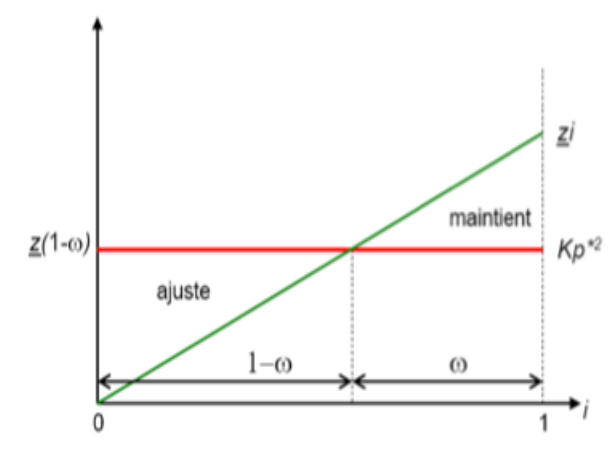
\includegraphics[width=11cm, height=8cm]{pc3_assets/1.png}
\end{center}
\item On rappelle qu'on est au voisinage de l'\'{e}quilibre sym\'{e}trique,
de sorte que log du prix moyen est en premi\`{e}re approximation \'{e}gal 
\`{a} la moyenne des prix en log. Avec  $p^{n}=0$ on a donc : 
\begin{equation*}
p=\int_{0}^{1}p_{i}\text{d}i=\omega p^{n}+\left( 1-\omega \right) p^{\ast
}=\left( 1-\omega \right) p^{\ast }
\end{equation*}%
o\`{u}%
\begin{equation*}
p^{\ast }=\frac{1}{\xi }y+p=y+p
\end{equation*}%
On obtient ainsi :%
\begin{equation*}
p=\left( 1-\omega \right) \left( y+p\right) =\left( \frac{1-\omega }{\omega }%
\right) y
\end{equation*}%
\textbf{Interpr\'{e}tation} : un niveau de production ($y$) \'{e}lev\'{e}
est associ\'{e} \`{a} des co\^{u}ts salariaux ($w-p$) \'{e}lev\'{e}s, ce qui
fait monter le prix de vente des firmes qui ajustent leur prix ($p^{\ast }$)
et donc le niveau g\'{e}n\'{e}ral des prix ($p$). L'impact sur le niveau g%
\'{e}n\'{e}ral des prix est d'autant plus important que le nombre de firmes 
\`{a} prix fixes ($\omega $) est faible.

\item On part des relations%
\begin{eqnarray}
1-\omega &=&\left( \frac{K}{\bar{z}}\right) p^{\ast 2}  \\
p &=&\left( 1-\omega \right) p^{\ast }  \\
p &=&\left( \frac{1-\omega }{\omega }\right) y 
\end{eqnarray}%
\newline
(9) et (10) permettent d'\'{e}liminer $p^{\ast }$ :%
\begin{equation*}
1-\omega =\left( \frac{K}{\bar{z}}\right) \left( \frac{p}{1-\omega }\right)
^{2}\Rightarrow \left( 1-\omega \right) ^{3}=\left( \frac{K}{\bar{z}}\right)
p^{2}
\end{equation*}%
soit%
\begin{equation*}
1-\omega \left( p\right) =\left( \frac{K}{\bar{z}}\right) ^{\frac{1}{3}%
}\left\vert p\right\vert ^{\frac{2}{3}}\text{ \ \ et \ \ }\omega \left(
p\right) =1-\left( \frac{K}{\bar{z}}\right) ^{\frac{1}{3}}\left\vert
p\right\vert ^{\frac{2}{3}}
\end{equation*}%
(11) peut alors se r\'{e}\'{e}crire%
\begin{equation*}
y\left( p\right) =\left( \frac{\omega \left( p\right) }{1-\omega \left(
p\right) }\right) p=\left( \left( \bar{z}/K\right) ^{\frac{1}{3}}\left\vert
p\right\vert ^{-\frac{2}{3}}-1\right) p
\end{equation*}%
Avec $\bar{z}/K=1$ on obtient par exemple, dans le plan ($p,y$) :%

\begin{center}
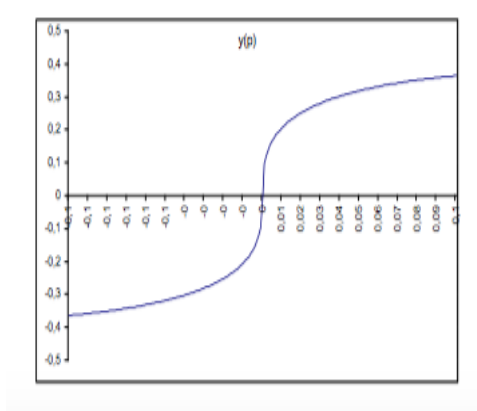
\includegraphics[width=9cm, height=7cm]{pc3_assets/2.png}
\end{center}

\begin{center}
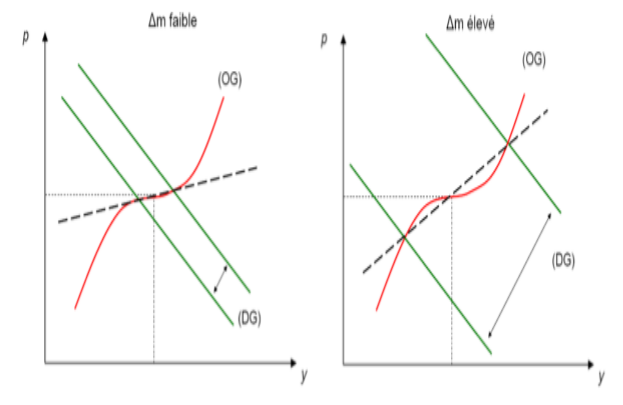
\includegraphics[width=11cm, height=8cm]{pc3_assets/3.png}
\end{center}


\bigskip
et donc l'inverse dans le plan ($y,p$)\bigskip \newline
Quand les chocs ($\Delta \theta$) sont faibles, la pente moyenne observ\'{e}e de
la courbe (OA) (telle que mesur\'{e}e par la droite des moindres carr\'{e}s,
par exemple) est faible, car peu de firmes ajustent leur prix suite \`{a} un
choc. A la limite, quand $\Delta \theta\rightarrow 0$ on a $y\rightarrow 0$ et la
pente de (OA) devient nulle (la proportion de firmes changeant ses prix tend
vers zero). Inversement, lorsque les chocs sont importants, la pente moyenne
observ\'{e}e est \'{e}lev\'{e}e car un plus grand nombre de firmes ajuste
ses prix suite \`{a} un choc. La pente moyenne observ\'{e}e de (OA) est donc
croissante de la volatilit\'{e} de la demande agr\'{e}g\'{e}e, tout comme
chez Lucas (1972, 1973). Une valeur de $\bar{z}$ \'{e}lev\'{e}e est associ%
\'{e}e \`{a} des co\^{u}ts de catalogue plus importants pour toutes les
firmes, ce qui r\'{e}duit la pente de (OA) pour toute valeur de $\Delta \theta $.
De la m\^{e}me mani\`{e}re, une valeur de $K$ \'{e}lev\'{e}e augmente le co%
\^{u}t d'opportunit\'{e} associ\'{e} au maintien d'un prix constant, ce qui r%
\'{e}duit la pente de (OA) pour toute valeur de $\Delta \theta$. On note que $%
K=\eta \left( \eta -1\right) /2$ est li\'{e} au degr\'{e} substituabilit\'{e}
entre les biens ($\eta $) et donc \`{a} l'intensit\'{e} de la concurrence
sur ce march\'{e}. Une concurrence plus forte tend \`{a} \'{e}lever la pente
de OA, et donc \`{a} r\'{e}duire l'impact des chocs mon\'{e}taires sur le
produit.\newline





\begin{center}
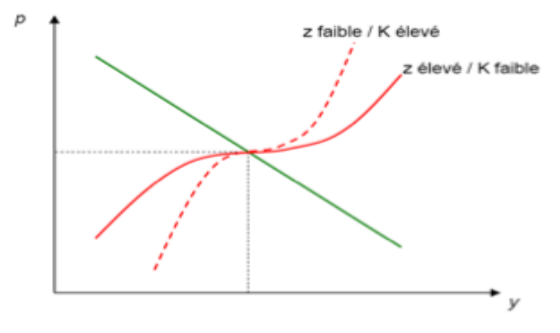
\includegraphics[width=11cm, height=6cm]{pc3_assets/4.png}
\end{center}

\item L'\'{e}quilibre apr\`{e}s le choc est caract\'{e}ris\'{e} par les \'{e}%
quations suivantes :%
\begin{eqnarray*}
p &=&\left( 1-\omega \right) p^{\ast }\text{ (prix moyen, avec }p^{n}=0\text{%
)} \\
p^{\ast } &=&\frac{1}{\xi }y+p\text{ (prix optimal, cf. question 3)} \\
y &=&\Delta \theta-p\text{ \ (demande agr\'{e}g\'{e}e avec }\theta_{1}=\Delta \theta\text{)}
\end{eqnarray*}%
Ce qui donne :%
\begin{eqnarray*}
p &=&\left( \frac{1-\omega }{1-\omega \left( 1-\xi \right) }\right) \Delta \theta
\\
y &=&\left( \frac{\omega \xi }{1-\omega \left( 1-\xi \right) }\right) \Delta
\theta \\
p^{\ast } &=&\left( \frac{1}{1-\omega \left( 1-\xi \right) }\right) \Delta \theta
\end{eqnarray*}



\item La perte proportionnelle de profit $Kp^{\ast 2}$ est donn\'{e}e par :%
\begin{equation*}
Kp^{\ast 2}=K\left( \frac{\Delta \theta}{1-\omega \left( 1-\xi \right) }\right)
^{2}
\end{equation*}%

Il est important de noter que $ p^{\ast} $ (d'où la perte de ne pas ajuster le prix) dépend de ce que font les autres entreprises lorsque $ \xi>1 $. Avec $\xi> 1 $ (offre de travail relativement \'{e}lastique), une hausse de $\omega $ diminue la perte  li\'{e}e au fait de maintenir un prix constant;
il y a donc des compl\'{e}mentarit\'{e}s strat\'{e}giques dans les d\'{e}cisions de prix. On dit qu'il y a des complémentarités stratégiques dans un jeu si l'incitation du joueur à entreprendre une certaine action est renforcée lorsque les autres joueurs font la même action. Nous verrons que dans ce modèle, les décisions des firmes de modifier les prix (ou de les maintenir inchangés) peuvent se renforcer mutuellement. Pour voir cela, utilisez (\ref{price}) pour obtenir




\begin{equation}\label{price2}
p^{\ast }=p\left(\frac{\xi-1}{\xi }\right) + \frac{\Delta \theta}{\xi} 
\end{equation}%


Cette équation montre que lorsque $ \xi>1$, nous avons que $p^{\ast}$ doit augmenter davantage si $ p $ augmente davantage. Autrement dit, si plus d'entreprises augmentent les prix après un choc $ \Delta \theta $, $ p $ croîtra davantage, de sorte que $ p^{\ast} $ devra croître davantage, poussant les entreprises à modifier les prix 

 


\begin{figure}[!tbp]
  \centering
  \begin{minipage}[b]{0.4\textwidth}
    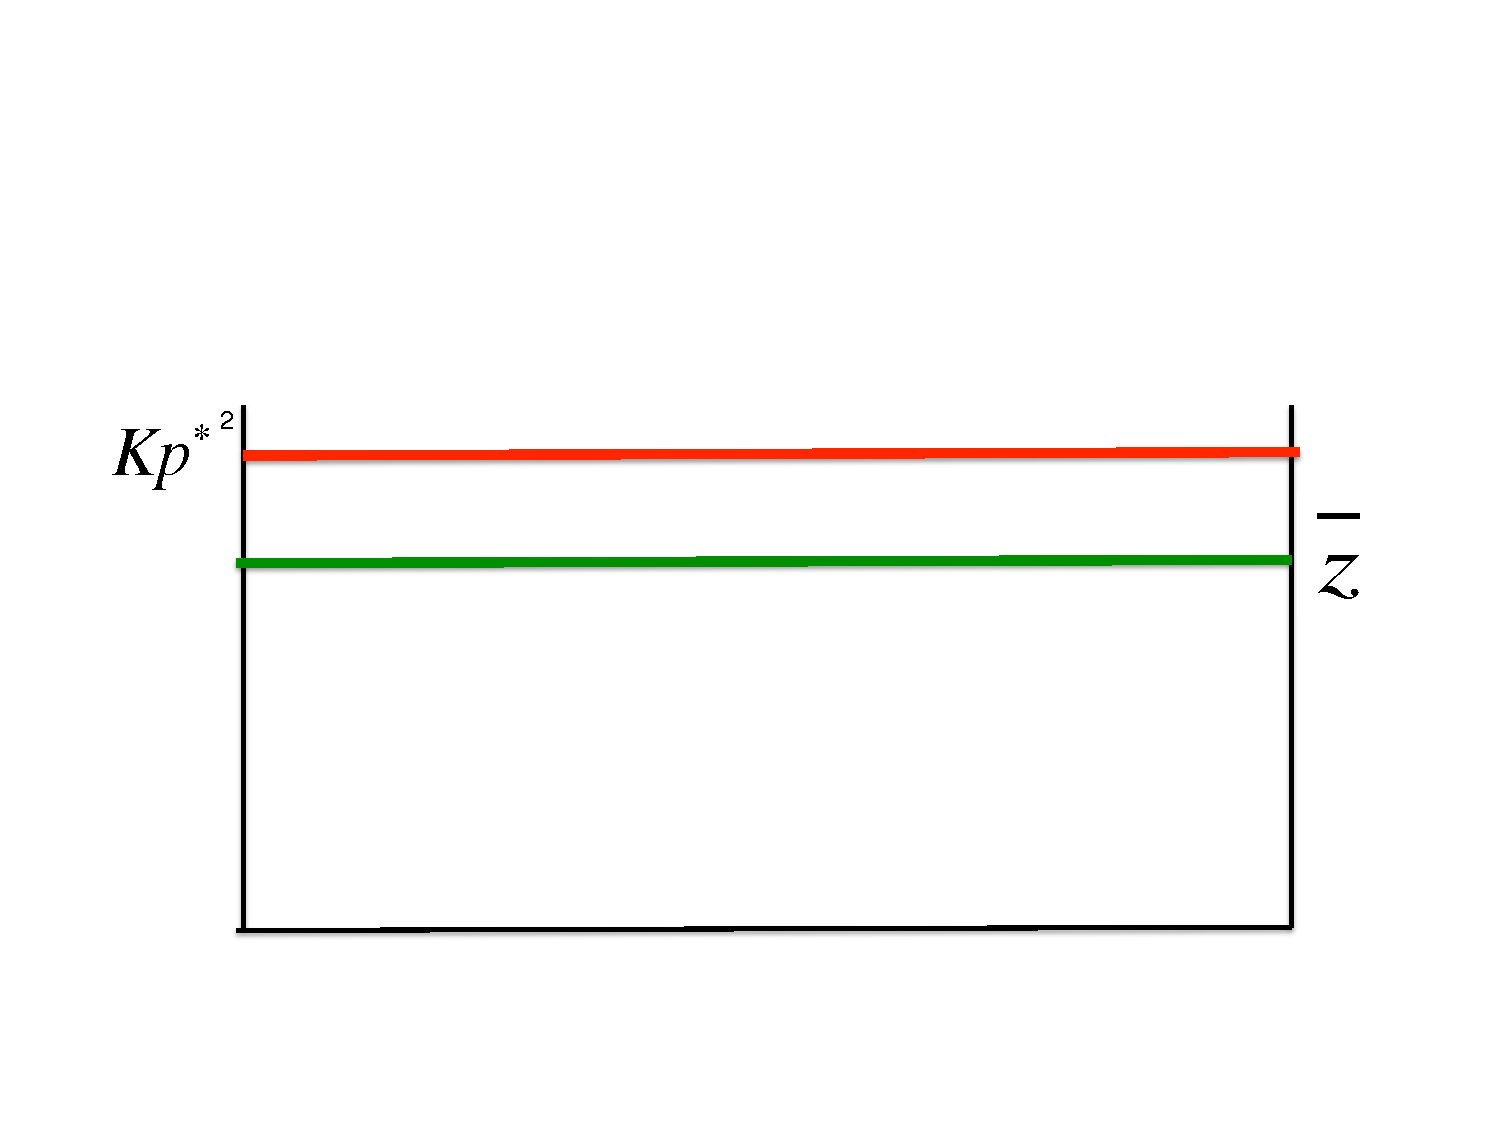
\includegraphics[width=1.3\textwidth]{pc3_assets/opti.pdf}
    \caption{perte de profit quand anticipation est $\omega =0$}
  \end{minipage}
  \hfill
  \begin{minipage}[b]{0.4\textwidth}
    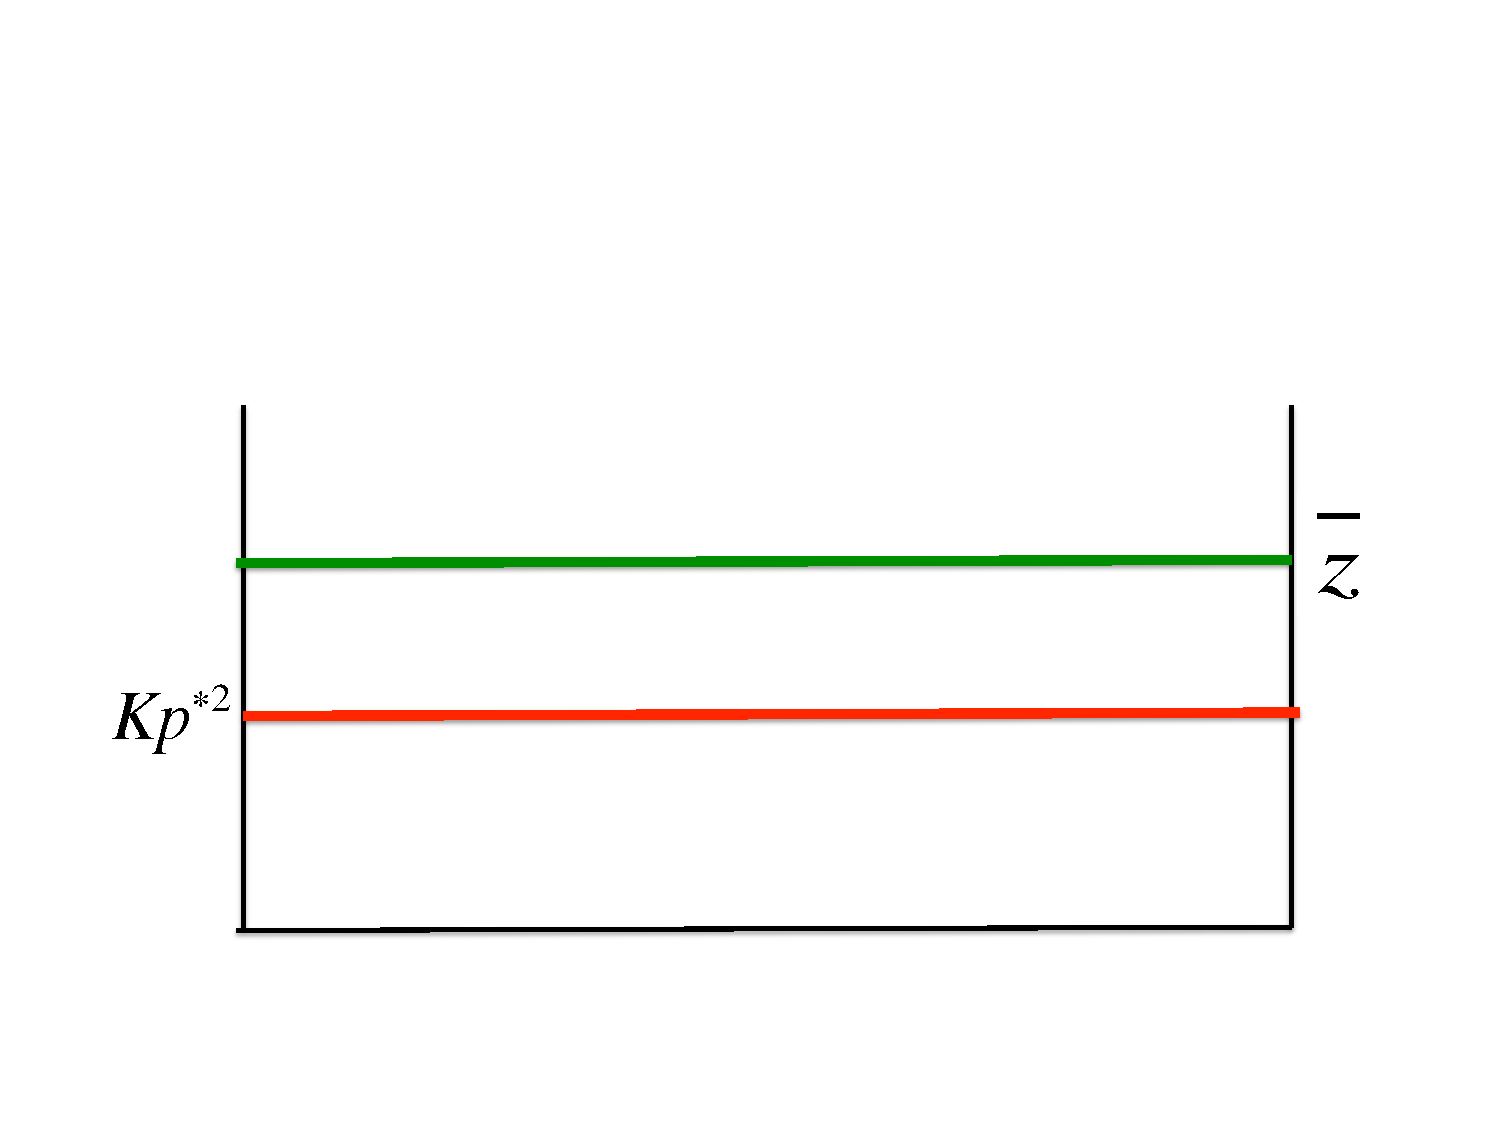
\includegraphics[width=1.3\textwidth]{pc3_assets/opt.pdf}
    \caption{perte de profit quand anticipation est $\omega =1$}
  \end{minipage}
\end{figure}

\item 

Contrairement à la deuxième partie, puisque le coût $\bar{z} $ est le même pour toutes les firmes, l'équilibre sera symétrique: soit  toutes les firmes changent de prix, soit toutes les firmes gardent le même prix.  Consid\'{e}rons les deux \'{e}quilibres potientiels tour \`{a} tour.
\end{enumerate}

\begin{itemize}
\item Supposons que chaque firme anticipe $\omega =1$. Cet \'{e}quilibre est
auto-r\'{e}alis\'{e} si la perte individuelle de profit (en niveau) associ%
\'{e}e au maintien d'un prix constant est inf\'{e}rieure au co\^{u}t de
catalogue :%
\begin{equation*}
Kp^{\ast 2}=K\left( \frac{%
\Delta \theta}{\xi }\right) ^{2}<\bar{z}\Leftrightarrow \left( \Delta \theta\right)
^{2}<\xi ^{2}\frac{\bar{z}}{K}
\end{equation*}

\item Supposons que chaque firme anticipe $\omega =0$. Cet \'{e}quilibre est
auto-r\'{e}alis\'{e} si la perte individuelle de profit associ\'{e}e au
maintien d'un prix constant est sup\'{e}rieure au co\^{u}t de catalogue : 
\begin{equation*}
Kp^{\ast 2}=K\left( \Delta \theta\right) ^{2}>\bar{z}\Leftrightarrow \left(
\Delta \theta\right) ^{2}>\frac{\bar{z}}{K}
\end{equation*}

\item Comme $\xi >1$, une multiplicit\'{e} d'\'{e}quilibres est possible
pour des valeurs int\'{e}rm\'{e}diaires de $\left( \Delta \theta\right) ^{2}$.
\end{itemize}

Dans la figure 1, nous avons que lorsque les entreprises s'attendent à ce que $ \omega = 0 $ (c'est-à-dire qu'aucune entreprise ne garde les prix inchangés), la perte de ne pas changer les prix (la ligne rouge) est supérieure à $ \bar{z} $ (ligne verte ):   l'attente est confirmée et il est en effet optimal de modifier les prix pour toutes les entreprises. Dans la figure 2, nous avons que lorsque les entreprises s'attendent à ce que $ \omega = 1 $ (c'est-à-dire qu'aucune entreprise ne change de prix), la perte de ne pas changer les prix est inférieure à $ \bar{z} $: il est  optimal de maintenir les prix inchangés. La multiplicité des équilibres implique que le cas keynésien ($ \omega = 1 $) ou le cas classique ($ \omega = 0 $) sont tous deux possibles dans la même économie: le résultat dépend des anticipations. Les anticipations auto-réalisatrices ont des conséquences sur la production: dans le cas keynésien, le choc DA a un effet potentiellement important sur la production car les entreprises ne changent pas de prix. Dans le cas classique, le choc n'a aucun effet sur la production, car les entreprises réagissent en modifiant les prix et non les quantités. Enfin, notez que les équilibres multiples ne se produisent pas lorsque les chocs $ \Delta \theta $ sont soit très élevés, soit très faibles. Dans le premier cas, toutes les entreprises changent de prix indépendamment des attentes. Dans le second cas, toutes les entreprises maintiennent les prix inchangés quelles que soient leurs attentes.

\newpage

\bigskip

\textbf{Perte de profit}

\bigskip

Soit $\Theta \left( X_{i}\right) $ le profit d'une firme qui vend au prix r%
\'{e}el $X_{i}=P_{i}/P$ : 
\begin{equation*}
\Theta \left( X_{i}\right) =YX_{i}^{-\eta }\left( X_{i}-\frac{W}{P}\right) ,
\end{equation*}%
avec $\Theta \left( X^{\ast }\right) $ le profit d'une firme qui vend au
prix r\'{e}el optimal. Pour $X_{i}$ proche de $X^{\ast }$ on a :%
\begin{equation*}
\Theta \left( X_{i}\right) -\Theta \left( X^{\ast }\right) \simeq \underset{%
=0\text{ (CPO)}}{\underbrace{\left. \frac{\partial \Theta \left(
X_{i}\right) }{\partial X_{i}}\right\vert _{X_{i}=X^{\ast }}}}\left(
X_{i}-X^{\ast }\right) +\frac{1}{2}\left. \frac{\partial ^{2}\Theta \left(
X_{i}\right) }{\partial X_{i}^{2}}\right\vert _{X_{i}=X^{\ast }}\left(
X_{i}-X^{\ast }\right) ^{2}
\end{equation*}%
soit%
\begin{equation*}
\frac{\Theta \left( X_{i}\right) -\Theta \left( X^{\ast }\right) }{\Theta
\left( X^{\ast }\right) }\simeq \underset{<0}{\underbrace{\left( \frac{%
X^{\ast 2}}{2\Theta \left( X^{\ast }\right) }\left. \frac{\partial
^{2}\Theta \left( X_{i}\right) }{\partial X_{i}^{2}}\right\vert
_{X_{i}=X^{\ast }}\right) }}\underset{\simeq x_{i}-x^{\ast }=p_{i}-p^{\ast }}%
{\underbrace{\left( \frac{X_{i}-X^{\ast }}{X^{\ast }}\right) }}^{2}
\end{equation*}%
o\`{u} $x_{i}=\ln X_{i}=p_{i}-p$. Ainsi, un \'{e}cart proportionnel au prix r%
\'{e}el optimal engendre une perte proportionnelle de profit de second
ordre. Pour mesurer la taille de cet effet, utilisons d'abord (\ref{Prix
reel optimal}) pour \'{e}crire le profit au prix optimal comme suit 
\begin{equation*}
\Theta \left( X_{i}\right) =YX_{i}^{-\eta }\left( X_{i}-\frac{W}{P}\right)
=YX_{i}^{-\eta }\left( X_{i}-\left( \frac{\eta -1}{\eta }\right) \frac{%
P^{\ast }}{P}\right)
\end{equation*}%
Ceci implique :%
\begin{eqnarray*}
\frac{\partial \Theta \left( X_{i}\right) }{\partial X_{i}} &=&-\eta
YX_{i}^{-\eta -1}\left( X_{i}-\left( \frac{\eta -1}{\eta }\right) \frac{%
P^{\ast }}{P}\right) +YX_{i}^{-\eta } \\
\frac{\partial ^{2}\Theta \left( X_{i}\right) }{\partial X_{i}^{2}} &=&\eta
\left( \eta +1\right) YX_{i}^{-\eta -2}\left( X_{i}-\left( \frac{\eta -1}{%
\eta }\right) \frac{P^{\ast }}{P}\right) -2\eta YX_{i}^{-\eta -1}
\end{eqnarray*}%
et donc%
\begin{equation*}
\left. \frac{\partial ^{2}\Theta \left( X_{i}\right) }{\partial X_{i}^{2}}%
\right\vert _{X_{i}=X^{\ast }}=\eta \left( \eta +1\right) Y\left( 1-\frac{%
\eta -1}{\eta }\right) -2\eta Y=Y\left( 1-\eta \right)
\end{equation*}%
Au voisinage de l'\'{e}quilibre sym\'{e}trique (o\`{u} $X^{\ast }\simeq 1$)
on a ainsi :%
\begin{equation*}
\frac{X^{\ast 2}\Theta ^{\prime \prime }\left( X^{\ast }\right) }{2\Theta
\left( X^{\ast }\right) }\simeq \frac{\left. \Theta ^{\prime \prime }\left(
X^{\ast }\right) \right\vert _{X^{\ast }=1}}{2\Theta \left( 1\right) }=\frac{%
Y\left( 1-\eta \right) }{2\frac{Y}{\eta }}=\frac{\eta \left( 1-\eta \right) 
}{2}<0
\end{equation*}%
La perte proportionnelle de profit s'\'{e}crit donc%
\begin{equation*}
K\left( p_{i}-p^{\ast }\right) ^{2}\text{, avec }K=-\frac{\eta \left( 1-\eta
\right) }{2}>0.
\end{equation*}%
Plus les biens sont substituables entre eux (c'est-\`{a}-dire plus $\eta $
est \'{e}lev\'{e}), plus l'intensit\'{e} de la concurrence augmente et plus
il devient co\^{u}teux de s'\'{e}carter du prix optimal $p^{\ast }$.

\end{document}
\bigskip
Soit $\Theta \left( P_{i}\right) $ le profit d'une firme qui vend au prix $P_{i}$ : 
\begin{equation*}
\Theta \left( P_i\right) =Y\left(\frac{P_i}{P}\right)^{-\eta }\left( P_{i}-W \right) ,
\end{equation*}%
avec $\Theta \left( P^{\ast }\right) $ le profit d'une firme qui vend au
prix r\'{e}el optimal. Pour $P_{i}$ proche de $P^{\ast }$ on a :%
\begin{equation*}
\Theta \left( P_{i}\right) -\Theta \left( P^{\ast }\right) \simeq \underset{%
=0\text{ (CPO)}}{\underbrace{\left. \frac{\partial \Theta \left(
P_{i}\right) }{\partial P_{i}}\right\vert _{P_{i}=P^{\ast }}}}\left(
P_{i}-P^{\ast }\right) +\frac{1}{2}\left. \frac{\partial ^{2}\Theta \left(
P_{i}\right) }{\partial P_{i}^{2}}\right\vert _{P_{i}=P^{\ast }}\left(
P_{i}-P^{\ast }\right) ^{2}
\end{equation*}%
soit%
\begin{equation}
\frac{\Theta \left( P_{i}\right) -\Theta \left( P^{\ast }\right) }{\Theta \left( P^{\ast}\right)}\simeq \underset{<0}{\underbrace{\left( \frac{%
P^{\ast 2}}{2\Theta \left( P^{\ast}\right) }\left. \frac{\partial
^{2}\Theta \left( P_{i}\right) }{\partial P_{i}^{2}}\right\vert
_{P_{i}=P^{\ast }}\right) }}\underset{\simeq p_{i}-p^{\ast }}%
{\underbrace{\left( \frac{P_{i}-P^{\ast }}{P^{\ast }}\right) }}^{2}\label{mess}
\end{equation}%
Ainsi, un \'{e}cart proportionnel au prix r%
\'{e}el optimal engendre une perte  de profit de second
ordre. 

\bigskip

\textbf{AR:} Since I changed  a bit the notation, I need to verify the algebra below. But I am thinking about not not including it in the solution key. )


\bigskip


Pour mesurer la taille de cet effet, utilisons d'abord (\ref{Prix
reel optimal}) pour \'{e}crire le profit au prix optimal comme suit 
\begin{equation*}
\Theta \left( P_{i}\right) =Y \left(\frac{P_{i}}{P}\right)^{-\eta }\left( P_{i}- W\right)
=Y\left(\frac{P_{i}}{P}\right)^{-\eta }\left( P_{i}-\left( \frac{\eta -1}{\eta }\right) %
P^{\ast }\right)
\end{equation*}%
Ceci implique :%
\begin{eqnarray*}
\frac{\partial \Theta \left( P_{i}\right) }{\partial P_{i}} &=&-\frac{\eta}{P}
Y\left(\frac{P_{i}}{P}\right)^{-\eta -1}\left( P_{i}-\left( \frac{\eta -1}{\eta }\right) %
P^{\ast }\right) +Y\left(\frac{P_{i}}{P}\right)^{-\eta } \\
\frac{\partial ^{2}\Theta \left( P_{i}\right) }{\partial P_{i}^{2}} &=&\frac{\eta}{P^2}
\left( \eta +1\right) Y\left(\frac{P_{i}}{P}\right)^{-\eta -2}\left( P_{i}-\left( \frac{\eta -1}{%
\eta }\right) P^{\ast }\right) -2\frac{\eta}{P} Y \left(\frac{P_{i}}{P}\right)^{-\eta -1}
\end{eqnarray*}%
et donc%
\begin{equation*}
\left. \frac{\partial ^{2}\Theta \left( P_{i}\right) }{\partial P_{i}^{2}}%
\right\vert _{P_{i}=P^{\ast }}=\eta \left( \eta +1\right) \frac{Y}{P}\left( 1-\frac{%
\eta -1}{\eta }\right) -2\eta Y=\frac{Y}{P}\left( 1-\eta \right)
\end{equation*}%





Au voisinage de l'\'{e}quilibre sym\'{e}trique (o\`{u} $P^{\ast }\simeq P$)
on a ainsi 
 $\Theta \left( P^{\ast}\right)=YP^{\ast}/\eta$ 
 
\begin{equation*}
\frac{P^{\ast 2}\Theta ^{\prime \prime }\left( P^{\ast }\right) }{2 \Theta \left( P^{\ast}\right)}\simeq \frac{\eta  (1-\eta) }{2 }<0
\end{equation*}%
La perte proportionnelle de profit s'\'{e}crit donc%
\begin{equation*}
K\left( p_{i}-p^{\ast }\right) ^{2}\text{, avec }K=-\frac{\eta \left( 1-\eta
\right) }{2}>0.
\end{equation*}%
Plus les biens sont substituables entre eux (c'est-\`{a}-dire plus $\eta $
est \'{e}lev\'{e}), plus l'intensit\'{e} de la concurrence augmente et plus
il devient co\^{u}teux de s'\'{e}carter du prix optimal $p^{\ast }$.


\end{document}

